In \autoref{chap:theory}, I introduced the theory of validators using the QAC
language family.  I also shown how to prove validators' correctness with a
simple $\Prog$ language.

However, in real-world testing practices, there are more problems to consider.
For example: How to interact with the SUT via multiple channels?  How to handle
external nondeterminism?

This chapter describes how to build tester programs that can interact with the
SUT and reveal potential defects.  \autoref{sec:itree} introduces the ITree
language for specifying protocols.  \autoref{sec:external-nondet} addresses
external nondeterminism by specifying the environment.
\autoref{sec:spec-to-test} explains the derivation mechanism from ITree
specifications to interactive tester programs, with an \http example.

\section{ITree Specification Language}
\label{sec:itree}
To write specifications for protocols' rich semantics, I employed ``interaction
tree'' (ITree), a generic data structure for representing interactive programs
in the Coq programming language, introduced by \textcite{itree}.  ITree allows
specifying protocols as monadic programs that model valid implementations'
possible behavior.  The model program can be interpreted into a tester program,
to be discussed in \autoref{sec:spec-to-test}.

\subsection{Language definition}
\label{sec:itree-lang}
Consider an echo program, which keeps reading some data and writing it out
verbatim, until reaching EOF:
\begin{lstlisting}[style=customcoq]
  CoInductive echo := c <- getchar;;
                      if c is EOF then EXIT
                      else putchar c;; echo.
\end{lstlisting}

Here the behavior after \ilc{read} depends on the value actually read.  This
monadic computation can be desugarized into:
\begin{lstlisting}[style=customcoq]
  CoInductive echo2 :=
    Bind getchar (fun c => if c is EOF then EXIT
                         else Bind (putchar c) (fun _ => echo)).
\end{lstlisting}

\begin{figure}
\begin{lstlisting}[style=customcoq]
  CoInductive itreeM (E: Type -> Type) (R: Type) :=
    Ret     : R   -> itreeM E R
  | Trigger : E R -> itreeM E R
  | Bind    : forall {X : Type}, itreeM E X -> (X -> itreeM E R) -> itreeM E R.
\end{lstlisting}
\caption{Mock definition of interaction trees.}
\label{fig:mock-itree}
\end{figure}

\begin{figure}
  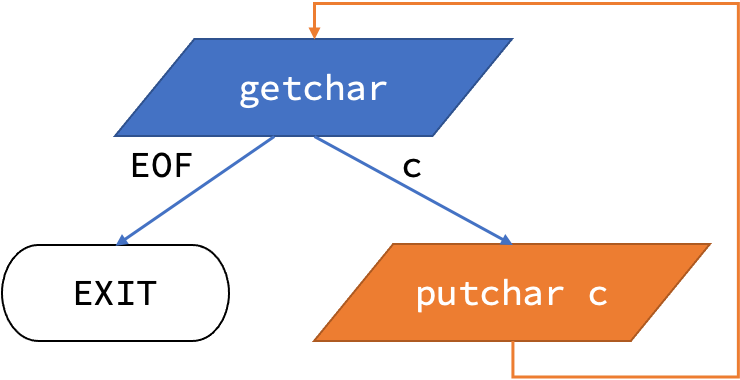
\includegraphics[width=.5\linewidth]{figures/echo-itree}
  \caption{Interaction tree for echo program}
  \label{fig:echo-itree}
\end{figure}

Such continuation-passing style can be represented as a tree of interactions.
To help readers better understand the interaction tree language, I first provide
a modified version of it that better shows its tree structure.

\paragraph{Mock interaction trees}
As shown in \autoref{fig:mock-itree}, a mock interaction tree (\ilc{itreeM}) has
two kinds of nodes, \ilc{Ret} and \ilc{Trigger}, and has edges constructed by
\ilc{Bind}:
\begin{itemize}
\item \ilc{(Ret r)} represents a pure computation that yields a value \ilc r.
  In the echo example, \ilc{EXIT} halts the program with return value zero:
\begin{lstlisting}[style=customcoq]
  Definition EXIT {E} : itreeM E Z := Ret 0.
\end{lstlisting}
\item \ilc{(Trigger e)} performs an impure event \ilc e and returns its result.
  Here \ilc{(e: E R)} is an event whose result is of type \ilc R.  For example,
  \ilc{getchar} has result type \ilc{char}, and \ilc{putchar}'s result type is
  \ilc{unit} (which corresponds to \inlinec{void} in C/C++, or \ilc{()} in
  Haskell).  These effective programs are constructed by triggering standard I/O
  events:
\begin{lstlisting}[style=customcoq]
  Variant stdioE: Type -> Type := (* event type *)
    GetChar:         stdioE char
  | PutChar: char -> stdioE unit.
  
  Definition getchar : itreeM stdioE char := Trigger GetChar.
  Definition putchar (c: char) : itreeM stdioE unit
                               := Trigger (PutChar c).
\end{lstlisting}
\item \ilc{(Bind m k)} binds the return value of \ilc m to the continuation
  function \ilc k.  It first runs program \ilc m until it returns some value of
  type \ilc X.  The return value \ilc{(x: X)} then instantiates \ilc k into the
  following computation \ilc{(k x: itreeM E R)}.  This corresponds to the
  \ilc{(;;)} syntax in \ilc{echo}:
\begin{lstlisting}[style=customcoq]
  Notation "x <- m1;; m2" := (Bind m1 (fun x => m2)).
  Notation "m1;; m2"      := (Bind m1 (fun _ => m2)).
\end{lstlisting}

As illustrated in \autoref{fig:echo-itree}, each possible return value \ilc x is
an edge that leads to the child it instantiates {\it i.e.} \ilc{(k x)}.  In this
way, the \ilc{Ret} and \ilc{Trigger} nodes are connected into a tree
structure.
\end{itemize}

The mock interaction tree provides an intuitive continuation-passing structure
for representing impure programs.  However, this language is not suitable for
writing specifications and deriving them into tester programs, because the test
derivation requires analyzing and transforming the specification program.

A mock interaction tree has infinitely many syntactic variants that are
semantically equivalent, due to monad laws.  For example, consider the following
programs:
\begin{lstlisting}[style=customcoq]
  Example bindret  r k     := Bind (Ret r) k.
  Example bindbind m k1 k2 := Bind (Bind m k1) k2.
\end{lstlisting}
These programs are semantically equivalent to:
\begin{lstlisting}[style=customcoq]
  Example bindret2  r k     := k r.
  Example bindbind2 m k1 k2 := x <- m;; Bind (k1 x) k2.
\end{lstlisting}

To make program analysis more effective, we need to redefine the tree structure
in a normal form, where each semantics corresponds to a unique syntax.

\paragraph{Actual interaction trees}
\begin{figure}
\begin{lstlisting}[style=customcoq]
  CoInductive itree (E: Type -> Type) (R: Type) :=
    Pure   : R -> itree E R
  | Impure : forall {X : Type}, E X -> (X -> itree E R) -> itree E R.
\end{lstlisting}
\caption{Formal definition of interaction trees}
\label{fig:itrees}
\end{figure}
The type defiinition of ITree restricts that only single events can be bound to
a continuation.  As shown in \autoref{fig:itrees}, we use \ilc{(Impure e k)} to
replace \ilc{(Bind (Trigger e) k)} representations in \ilc{itreeM}.  A
\ilc{Pure} computation cannot be bound to a continuation, and must be the leaf
of an ITree.

The \ilc{Ret}, \ilc{Trigger}, and \ilc{Bind} constructors introduced in
\ilc{itreeM} have equivalent representations in \ilc{itree}, so we can still
write programs monadically with \ilc{(;;)} :
\begin{lstlisting}[style=customcoq]
  Definition ret {E R} : R -> itree E R := Pure.
  
  Definition trigger {E R} (e: E R) : itree E R := Impure e Pure.

  CoFixpoint bind {X E R} (m: itree E X) (f: X -> itree E R) : itree E R :=
    match m with
    | Pure   x   => f x
    | Impure e k => Impure e (fun r => bind (k r) f)
    end.

  Notation "x <- m1;; m2" := (bind m1 (fun x => m2)).
  Notation "m1;; m2"      := (bind m1 (fun _ => m2)).

  CoFixpoint translateM {E R} (m: itreeM E R) : itree E R :=
    match m with
    | Ret     r => ret r
    | Trigger e => trigger e
    | Bind m1 k => x <- translate m1;; translate (k x)
    end.
\end{lstlisting}

ITrees can specify various kinds of programs like servers and testers, by
defining different event types.  For example, the QAC server in
\autoref{def:server} exhibits internal nondeterminism.  The internal choices
made by the server can be represented as \ilc{Choice} events whose result can be
any value in the space of choices:
\begin{lstlisting}[style=customcoq]
  Variant choiceE: Type -> Type :=
    Choice: choiceE C.
\end{lstlisting}

The server also needs to send requests and receive responses:
\begin{lstlisting}[style=customcoq]
  Variant qaE: Type -> Type :=
    Recv: qaE Q           (* receive a request *)
  | Send: A -> qaE unit.  (* send a response   *)

  Definition qacE: Type -> Type := qaE +' choiceE.
\end{lstlisting}

Here \ilc{qacE} is a sum type of \ilc{qaE} and \ilc{choiceE} events, meaning
that the server may send or receive messages, and may also make internal
choices.  We split the event types because they'll be handled differently when
we derive the tester later in this chapter.

Now we can represent the QAC server with step function \ilc{sstep} and initial
state \ilc S:
\begin{lstlisting}[style=customcoq]
  CoInductive server (sstep: Q -> C -> S -> A * S) (s: S)
              : itree qacE void :=
    c <- trigger Choice;;
    q <- trigger Recv;;
    let (a, s') := sstep q c s in
    trigger (Send a);;
    server sstep s'.
\end{lstlisting}

This subsection has provided a brief taste of the ITree specification language.
To construct a tester from the specification, we need to dualize the model's
behavior into the tester-side behavior, based on the theory explained in
\autoref{sec:dualization}.  To dualize specifications written in ITrees, we need
an {\em interpretation} mechanism that transforms ITrees into other programs,
which will be explained in the next subsection.

\subsection{Interpreting interaction trees}
To interpret a program \ilc p is to specify a rule that defines ``if \ilc p does
this, then do that''.  For example, shell syntax \inlinec{(p < input > output)}
executes \inlinec p but redirects its standard I/O.  Suppose \inlinec p is the
\ilc{echo} program in \autoref{sec:itree-lang}, then the redirected program
should perform file operations:
\begin{lstlisting}[style=customcoq]
  Variant fileE: Type -> Type :=      (* file operation events *)
    Fgetc: file ->         fileE char
  | Fputc: file -> char -> fileE unit.

  CoInductive redirect_echo (input output: file) : itree fileE unit :=
    c <- trigger (Fgetc input);;
    if c is EOF then ret 0
    else trigger (Fputc output c);;
         redirect_echo input output.
\end{lstlisting}

The interpretation rule is ``whenever the program wants to read from or write to
standard IO, perform the read/write operation on the specified file instead'':
\begin{lstlisting}[style=customcoq]
  Definition redirect (input output: file) {R: Type} (e: stdioE R) :=
    match e in stdioE R return itree fileE R with
    | GetChar   => trigger (Fgetc input)
    | PutChar c => trigger (Fputc output c)
    end.
\end{lstlisting}

Here the \ilc{redirect} function takes a standard I/O event and turns it into an
ITree program that performs file events.  The result program has the same return
type as the original event, so it can ``replace'' the original \ilc{stdioE}.
This is done by the \ilc{interp} function:
\begin{lstlisting}[style=customcoq]
  CoFixpoint interp {E F R} (f: forall {T}, E T -> itree F T) (m: itree E R)
             : itree F R :=
    match m with
    | Pure   r   => Pure r
    | Impure e k => x <- f e;;
                    interp handler (k x)
    end.

  Definition redirect_echo2 (input output: file) : itree fileE unit :=
    interp (redirect input output) (translateM echo).
\end{lstlisting}

For each impure event, the interpretor replaces it with the program defined by
the handler function \ilc f.  As a result, \ilc{redirect_echo2} constructs a
redirected echo program that is equivalent with \ilc{redirect_echo}.

To derive tester programs from ITree specifications, I'll introduce multiple
interpretation processes, with various event handlers throughout this chapter.

\section{Handling External Nondeterminism}
\label{sec:external-nondet}
As introduced in \autoref{sec:intro-external-nondet}, the environment might
affect the transmission of messages, so called external nondeterminism.  The
tester should take the environment into account when validating its
observations.

This section explains how to address external nondeterminism by specifying the
environment, with the networked server example.  \autoref{sec:net-tcp} defines a
model for concurrent TCP connections.  \autoref{sec:net-compose} then composes
the network model with the server specification, yielding a tester-side
specification that defines the space of valid observations.

\subsection{Modelling the network}
\label{sec:net-tcp}
When testing servers over the network, request and response packets may be
indefinitely delayed.  As a result, messages from one end might arrive at the
other end in a different order from that they were sent.

The space of network reorderings can be modelled by a {\em network model}, a
conceptual program for the ``network wire''.  The wire can be viewed as a
buffer, which absorbs packets and later emits them:
\begin{lstlisting}[style=customcoq]
  Variant netE: Type -> Type := (* network event type *)
    Emit  : packet -> netE unit
  | Absorb: netE packet.
\end{lstlisting}

After absorbing a packet, the wire may emit it immediately or after
absorbing/emitting other packets.  Such choices are modelled by nondeterministic
\ilc{Or} branches:
\begin{lstlisting}[style=customcoq]
  Variant nondetE: Type -> Type := (* nondeterministic branch *)
    Or: nondetE bool.

  Definition or {E R} `{nondetE -< E} (x y: itree E R) : itree E R :=
    b <- trigger Or;;
    if b then x else y.
\end{lstlisting}

Here \ilc{(or x y)} creates a nondeterministic program that may behave as either
\ilc x or \ilc y.  The \ilc{nondetE} here is a special case of \ilc{choiceE}
defined in \autoref{sec:itree-lang} with boolean space of choices, but they'll
be handled differently during test derivation.  The type signature \ilc{\{E R\}
  `\{nondetE -< E\}} says the \ilc{(or)} combinator can apply to ITrees whose
event \ilc E is a super-event of \ilc{nondetE}, and with arbitrary return type
\ilc R.  For example, arguments \ilc x and \ilc y can be of type \ilc{(itree
  (netE +' nondetE) void)}.

For example, the network model for concurrent TCP connections is defined in
\autoref{fig:tcp-model}.  The model captures TCP's feature of maintaining the
order within each connection, but packets in different connections might be
reordered arbitrarily.  When the wire chooses a packet to send, the candidate
must be the oldest in its connection.

\begin{figure}
\begin{lstlisting}[style=customcoq]
Fixpoint pick_one (l: list packet) : itree nondetE (option packet) :=
  if l is p::l'
  then or (Ret (Some p)) (pick_one l')
  else ret None.

Definition oldest_in_each_conn : list packet -> list packet := ...
(* filter the oldest packet in each connection *)

CoFixpoint tcp (buffer: list packet) : itree (netE +' nondetE) void :=
  let absorb := pkt <- trigger Absorb;;
                tcp (buffer ++ [pkt])      in
  let emit p := trigger (Emit p);;
                tcp (remove pkt buffer)    in
  let pkts   := oldest_in_each_conn buffer in
  opkt <- pick_one pkts;;
  if opkt is Some pkt
  then emit pkt
  else absorb.
\end{lstlisting}
\caption[Network model for concurrent TCP connections]{Network model for
  concurrent TCP connections.  The model is an infinite program iterating over a
  \ilc{buffer} of all packets en route.  In each iteration, the model either
  \ilc{absorb}s or \ilc{emit}s some packet, depending on the current
  \ilc{buffer} state and the choice made in \ilc{pick_one}.  Any absorbed packet
  is appended to the end of buffer.  When emitting a packet, the model may
  choose a connection and send the oldest packet in it.}
\label{fig:tcp-model}
\end{figure}

Notice the \ilc{pick_one} function, which might return (i) \ilc{Some p} or (ii)
\ilc{None}.  \lys{Should I explain what is option type?}  The network model then
(i) emits packet \ilc p or (ii) absorbs a packet into \ilc{buffer}.

\begin{itemize}
\item When the given list \ilc{pkts} is empty, \ilc{pick_one} always returns
  \ilc{None}, becuase the wire has no packet in the \ilc{buffer}, and must
  absorb some packet before emitting anything.
\item Given a non-empty linked list \ilc{(p::l')}, with \ilc p as head and
  \ilc{l'} as tail, \ilc{pick_one} might return \ilc{(Some p)}, meaning the wire
  can emit that packet; or it might return \ilc{None}, meaning the wire can
  still absorb packets into the buffer.
\end{itemize}

Such network model reflects the TCP environment, where messages are never lost
but might be indefinitely delayed.  In the next subsection, I'll demonstrate how
to compose the server and network models into a client-side observation model.

\subsection{Network composition}
\label{sec:net-compose}

The network connects the server on one end to the clients on other ends.  When
one end sends some message, the network model absorbs it and later emits it to
the destination.

To {\em compose} a server model with a network model is to pair the server's
\ilc{Send} and \ilc{Recv} events with the network's \ilc{Absorb} and \ilc{Emit}
events.  Since the network model is nondeterministic, it might not be ready to
absorb packets sent by the server.  The network might also emit a packet before
the server is ready to receive it.

\begin{figure}
  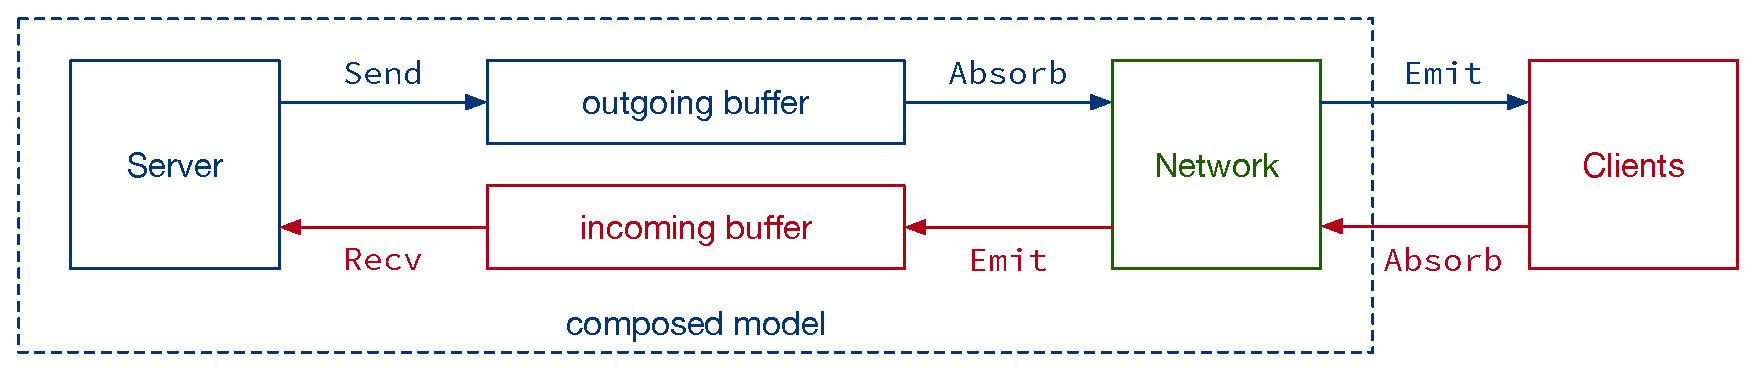
\includegraphics[width=\textwidth]{figures/net-compose}
  \caption{Network composition architecture}
  \label{fig:net-compose}
\end{figure}

To handle the asynchronicity among the server and network events, I insert
message buffers between them.  As shown in \autoref{fig:net-compose}, the {\em
  incoming buffer} stores the packets emitted by the network but not yet
consumed by the server's \ilc{Recv} events, and the {\em outgoing buffer} stores
the packets sent by the server but not yet absorbed by the network.

\begin{figure}
\begin{lstlisting}[style=customcoq,numbers=left,escapechar=\%]
CoFixpoint compose {E} (srv: itree (qaE +' E) void)   (* server  model *)
           (net  : itree (netE +' nondetE) void)      (* network model *)
           (bi bo: list packet)       (* incoming and outgoing buffers *)
           : itree (netE +' nondetE +' E) void :=
  let step_net :=%\label{line:step-net-def}%
    match net with
    | Impure Absorb knet =>
      if bo is pkt::bo'
      then compose srv (knet pkt) bi bo'%\label{line:net-absorb}%
      else pkt <- trigger Absorb;;%\label{line:client-send}%
           compose srv (knet pkt) bi bo
    | Impure (Emit pkt) knet =>
      if toServer pkt
      then compose srv (knet tt) (bi++[pkt]) bo%\label{line:srv-incoming}%
      else trigger (Emit pkt);;%\label{line:net-emit}%
           compose srv (knet tt) bi bo
    | Impure Or knet => b <- trigger Or;;
                        compose srv (knet b) bi bo
    | Pure vd => match vd in void with end
    end
  in
  match srv with
  | Impure Recv ksrv =>
    if bi is pkt::bi'
    then compose (ksrv pkt) net bi' bo%\label{line:srv-consume}%
    else step_net%\label{line:step-net}%
  | Impure (Send pkt) ksrv =>%\label{line:srv-send}%
    compose (ksrv tt) net bi (bo++[pkt])
  | Impure e ksrv =>           (* other events performed by the server *)
    r <- trigger e;; compose (ksrv r) net bi bo
  | Pure vd => match vd in void with end
  end.
\end{lstlisting}
\caption[Network composition algorithm]{Network composition algorithm.  When the
  server wants to send a packet in \autoref{line:srv-send}, the packet is
  appended to the outgoing buffer until absorbed by the network in
  \autoref{line:net-absorb}, and eventually emitted to the client in
  \autoref{line:net-emit}.  Conversely, packets sent by clients are absorbed by
  the network in \autoref{line:client-send}, emitted to the server's incoming
  buffer in \autoref{line:srv-incoming}, until the server consumes it in
  \autoref{line:srv-consume}.}
\label{fig:net-compose-code}
\end{figure}

The server and the clients are the opposite ends of the network.  Each packet
has routing fields that indicate its source and destination.  When the network
emits a packet, we need to determine whether the packet is emitted to the
server's incoming buffer or to the clients, by inspecting its destination:
\begin{lstlisting}[style=customcoq]
  Record packet := {
    source      : connection;
    destination : connection;
    payload     : data
  }.

  Definition toServer (p: packet) : bool :=
    if p.(destination) is server_conn then true else false.
\end{lstlisting}

Now we can define the composition algorithm formally, as shown in
\autoref{fig:net-compose-code}.  In this example, we reuse the \ilc{qaE}
definition in \autoref{sec:itree-lang}, and let the \ilc Q and \ilc A both be
the \ilc{packet} type.  The composed ITree takes the server and network models
as parameters, and makes steps in the two ITrees in certain order.  The composed
model exhibits to the client three kinds of events: (i) Network operations
(\ilc{netE}) where packets are emitted to or absorbed from clients, (ii)
Nondetermistic branches (\ilc{nondetE}) made by the network model, and (iii)
Other events \ilc{\{E\}} performed by the server model {\it e.g.} internal
choices (\ilc{choiceE}) in \autoref{sec:itree-lang}.

Notice that this algorithm schedules the server at a higher priority than the
network model.  The composed model only steps into the network model when the
server is starved in \autoref{line:step-net}, by calling the \ilc{step_net}
process defined in \autoref{line:step-net-def}.  Such design is to avoid
divergence of the derived tester program, which I'll further explain in
\autoref{sec:spec-to-test}.

So far I've shown how to specify systems that exhibit external nondeterminism.
By specifying the environment and composing it with the specification, we can
describe the space of valid observations.  The rest of this chapter will show
how to derive tester programs from these observer-side specifications.

\section{From Specification to Tester}
\label{sec:spec-to-test}

From the server and network models, I derived a tester client that interacts
with servers over the network, and validates the observations against the
protocol specification, as shown in \autoref{fig:framework}.

\begin{figure}
  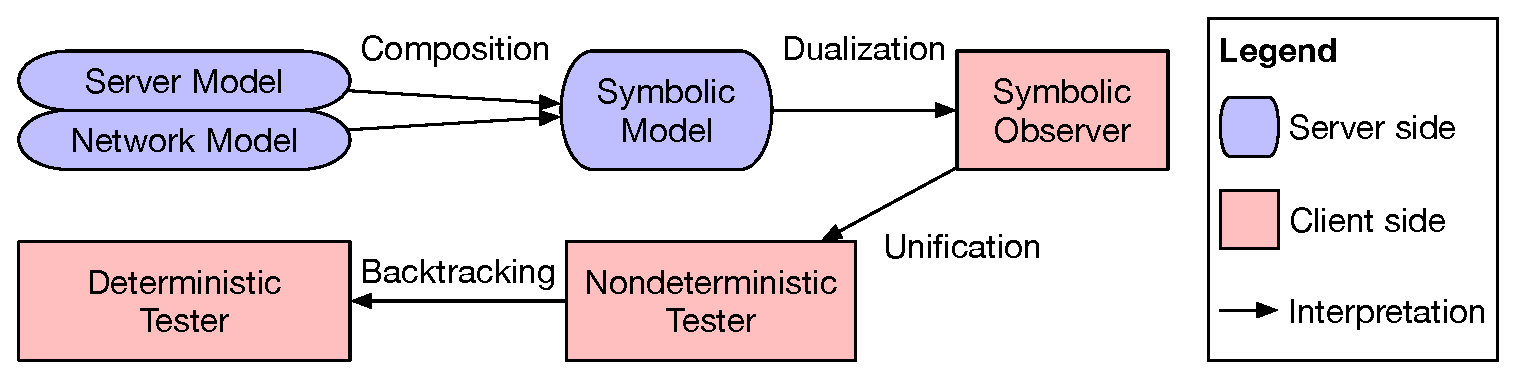
\includegraphics[width=\linewidth]{figures/framework}
  \caption{Deriving tester program from specification}
  \label{fig:framework}
\end{figure}

\subsection{Dualizing ITree model}
To {\em observe} the server's behavior, we have to interpret the specified
server-side events into tester-side events: When the server should send a
certain message, the tester expects to receive the specified message, and
rejects the server upon receiving an unexpected message; when the server should
receive some message, the tester generates a message and sends it to the server,
as shown in \autoref{fig:sym-observe}.

\begin{figure}
  \begin{lstlisting}[style=customcoq]
let observe (server) =
  match server with
  | pkt := recv(); s'(pkt) =>
    p := gen_pkt(); send(p); observe (s'(p))
  | send(pkt); s' =>
    p := recv(); guard(pkt, p); observe (s')
  | IF (x, s1, s2) =>
    (* Allow validating observation with [s1],
     * provided [x] is unifiable with [true];
     * Or, unify [x] with [false],
     * and validate observation with [s2]. *)
    determine(unify(x, true ); observe (s1),
              unify(x, false); observe (s2))
  | r  := _(); s'(r) =>
    r1 := _(); observe (s'(r1))
  end
  \end{lstlisting}
  \caption{Dualizing server model into observer model.  Upon \ilc{recv} events,
    the observer generates a packet and sends it to the server.  For \ilc{send}
    events, the observer receives a packet \ilc{p1}, and fails if it does not
    match the specified \ilc{pkt}.  When the server makes nondeterminstic
    \ilc{IF} branches, the observer \ilc{determine}s between the branches by
    \ilc{unify}ing the branch condition with its conjectured value, and then
    observing the corresponding branch.
    %% Such unification may fail immediately, or add a constraint to the
    %% symbolic variables in \ilc{x}, which instructs future
    %% observations. \bcp{??}
  }
  \label{fig:sym-observe}
\end{figure}

Besides sending and receiving messages, the model also has \ilc{IF} branches
conditioned over symbolic expressions, like that shown in
\autoref{fig:if-match-model}.  Upon nondeterministic branching, the tester needs to
determine which branch was actually taken, by constructing observers for both
branches.  Each branch represents a possible explanation of the server's
behavior.  Upon further interacting with the server, some branches might fail
because its conjecture cannot explain what it has observed.  The tester rejects
the server if all branches have failed, indicating that the server corresponds
to no possible case in the model.
%% \bcp{Very confusing.}

Dualizing the server-side model produces an observer model that performs
interactions to reveal the server's behavior and check its validity.  This model
includes all possible observations from a valid server, and needs to
\ilc{determine} which branch in the server model matches the observed behavior.
The model validates its observations with unification events \ilc{unify} and
\ilc{guard}.  These primitive events are handled by later interpretations: The
\ilc{unify} and \ilc{guard} events in each branch are instantiated into symbolic
evaluation logic that decides whether this branch should fail or not; The
\ilc{determine} events are instantiated into backtracking searches to find if
all branches have failed, which rejects the server.


\subsection{Symbolic Evaluation}

\begin{figure}
  \begin{lstlisting}[style=customcoq,numbers=left,escapechar=\%]
(* unifyS = list variable * list constraint    *)
(* new_var : unifyS -> variable * unifyS        *)
(* assert : exp T * T * unifyS -> option unifyS *)
let unifier (observer, map : mcid -> pcid,
         vars : unifyS) =
  match observer with
  | x := fresh(); o'(x) =>
    let (x1, vars') = new_var(vars) in
    unifier (o'(x1), vars', map)
  | unify(x, v); o' =>
    match assert(x, v, vars) with
    | Some vars' => unifier (o', vars', map)
    | None => failwith "Unexpected payload"
    end
  | guard(p0, p1); o' =>
    match assert(p0, p1, vars) with
    | Some vars' =>
      let mc = p0.source in %\label{line:begin-cid}%
      let pc = p1.source in
      if mc.is_created_by_server
      then match map[mc] with
           | pc => unifier (o', vars', map)
           | unknown =>
             let map' = update(map, mc, pc) in
             unifier (o', vars', map')
           | others =>
             failwith "Unexpected connection"
           end %\label{line:end-cid}%
      else unifier (o', vars', map)
    | None => failwith "Unexpected payload"
    end
  | r  := _(); o'(r) =>
    r1 := _(); unifier (o'(r1), vars, map)
  end\end{lstlisting}
  \caption{Instantiating symbolic events.  The tester maintains a \ilc{unifyS}tate
    which stores the constraints on symbolic variables.  When the
    specification creates a \ilc{fresh} symbol, the tester creates an entry for
    the symbol with no initial constraints.  Upon \ilc{unify} and
    \ilc{guard} events, the tester checks whether the \ilc{assert}ion is
    compatible with the current constraints.  If yes, it updates the constraints
    and move on; otherwise, it raises an error on the current branch.
    %% \sz{We should mention the \ilc{fresh} operation in the main text!}
  }
  \label{fig:unifier}
\end{figure}

In this interpretation phase, we handle nondeterminism at data level by handling
\ilc{fresh} events in the server model, as well as \ilc{unify} and \ilc{guard}
events introduced by dualization.  The interpretor instantiates these events
into symbolic evaluation algorithms.

As shown in \autoref{fig:unifier} (skip
\autoref{line:begin-cid}--\ref{line:end-cid} for now---we'll
explain that part later), the tester checks whether the observed/conjectured
value matches the specification, by maintaining the constraints on the symbolic
variables.  These constraints are initially empty when the variables are
generated by \ilc{fresh} events.  As the test runs into \ilc{unify} and
\ilc{guard} events, it adds constraints \ilc{assert}ing that the observed value
matches the specification, and checks whether the constraints are still
compatible.  Incompatibility among constraints indicates that the server has
exhibited behavior that cannot be explained by the model, implying violation
against the current branch of specification.

\subsection{Handling Incoming Connections}
In addition to generating data internally, the server might exhibit another kind
of nondeterminism related to the outgoing connections it creates.  For example,
when a client uses an HTTP server as proxy, requesting resources from another
server, the proxy server should create a new connection to the target server.
However, as shown in \autoref{fig:proxy-valid-trace}, when the tester receives a
request from an accepted connection, it does not know which client's
request the proxy was forwarding, due to network delays.

Outgoing connections created by the server model are identified by ``model
connection identifiers'' (\ilc{mcid}), and the tester accepts incoming
connections identified by ``physical connection identifiers'' (\ilc{pcid}).  As
shown in \autoref{line:begin-cid}--\ref{line:end-cid} of
\autoref{fig:unifier}, to determine which \ilc{mcid} in the specification does a
runtime \ilc{pcid} corresponds to, the tester maintains a \ilc{map}ping between
the connection identifiers.  Such mapping ensures the tester to check
interactions on an accepted connection against the right connection specified by
the server model.


\subsection{Backtracking}

\begin{figure}
  \begin{lstlisting}[style=customcoq,escapechar=\%]
(* filter : event T * T * list M -> list M *)
(* [filter(e, r, l)] returns a subset in [l],
 * where the model programs' next event is [e]
 * that returns [r]. *)
let backtrack (current, others) =
  match current with
  | determine(t1, t2) =>
    backtrack (t1, t2::others)
  | failwith error => (* current branch failed *) %\label{line:begin-failure}%
    match others with
    | [] => failwith error
    | another::ot' => backtrack (another, ot')
    end %\label{line:end-failure}%
  | send(pkt); t' =>
    let ot' = filter(SEND, pkt, others) in %\label{line:filter-send}%
    send(pkt); backtrack (t', ot')
  | pkt := recv(); t'(pkt) =>
    opkt := maybe_recv();
    match opkt with
    | Some p1 =>
      let ot' = filter(RECV, pkt, others) in %\label{line:filter-recv}%
      backtrack (t'(p1), ot')
    | None =>             (* no packet arrived *)
      match others with
      | [] => backtrack (current, []) (* retry *)
      | another::ot' =>            (* postpone *)
        backtrack (another, ot'++[current])
      end
    end
  end in
backtrack (tester_nondet, [])
  \end{lstlisting}
  \caption{From nondeterministic model to deterministic tester program.  If the
    model makes nondeterministic branches, the tester picks a branch to start
    with, and puts the other branch into a set of other possibilities.  If the
    current branch has failed, the tester looks for other possible branches to
    continue checking.  When the current branch sends a packet, the tester
    filters the set of other possibilities, and only keeps the branches that
    match the current send event.  If the model wants to receive a packet, the
    tester handles both cases whether some packet has arrived or not.}
  \label{fig:backtrack}
\end{figure}

Symbolic evaluation determines whether the observations matches the tester's
conjectures on each branch.  So far, the derived tester
is a nondeterministic program that rejects the server if and only if all
possible branches have raised some error.  To simulate this tester on a
deterministic machine, we execute one branch until it fails.  Upon failure in
the current branch, the simulator switches to another possible branch, until it
exhausts all possibilities and rejects the server, as shown in
\autoref{line:begin-failure}--\ref{line:end-failure} of
\autoref{fig:backtrack}.

When switching from one branch to another, the tester cannot revert its previous
interactions with the server.  Therefore, it must match the server model against
all interactions it has performed, and filter out the mismatching branches, as
shown in \autoref{line:filter-send} and \autoref{line:filter-recv} of
\autoref{fig:backtrack}.
%% , utilizing the lazy evaluation nature of our
%% specification language.\sz{Mention this earlier when introducing Galina?}

We've now derived a tester from the server model.  The specified server runs
forever, and so does the tester (upon no violations observed).  We accept the
server if the tester hasn't rejected it after some large, pre-determined number
of steps of execution.


\iffalse
\section{Specification Languages}

\subsection{Property-based specification with QuickChick}
My first formal specification of \http was written as
QuickChick~\cite{quickchick} properties, which takes a trace of requests, and
determines whether the traces is valid per protocol specification, like that
shown in \autoref{fig:etag-tester}.  The specification implemented a constraint
solving logic by hand, making it hard to scale when the protocol becomes more
complex, as discussed in \autoref{sec:challenges}

\subsection{Model-based specification with ITrees}

From an ITree specification, I conducted ``offline'' testing, which takes a
trace and determines its validity~\cite{cpp19}, and ``online'' testing, where
the specification is derived into a client program that validates the system
under test interactively~\cite{issta21}.

\subsection{Offline testing of swap server}
I started with testing a simple ``swap server''~\cite{cpp19}, specified in
\autoref{fig:linear-spec}.  The specification says that the server can either
accept a connection with a new client (\ilc{obs_connect}) or else receive a
message from a client over some established connection (\ilc{obs_msg_to_server}
\ilc{c}), send back the current stored message (\ilc{obs_msg_from_server}
\ilc{c} \ilc{last_msg}), and then start over with the last received message as
the current state.

To test this swap server, I wrote a client program that interacts with the
server and produces a trace of requests and responses, and a function that
determines whether the trace $t$ is a trace of the linear specification $s$ {\it
  i.e.} whether \ilc{is_trace s t} in \autoref{fig:itrees} holds.

To network nondeterminism, the checker enumerates all possible server-side
message orders that can explain the client-side observations, and checks if any
of them satisifes the protocol specification.
\begin{figure}
\begin{lstlisting}[style=customcoq]
  CoFixpoint linear_spec' (conns : list connection_id)
             (last_msg : bytes) : itree specE unit :=
    or ( (* Accept a new connection. *)
         c <- obs_connect;;
         linear_spec' (c :: conns) last_msg )
       ( (* Exchange a pair of messages on a connection. *)
         c <- choose conns;;
         msg <- obs_msg_to_server c;;
         obs_msg_from_server c last_msg;;
         linear_spec' conns msg ).

  Definition linear_spec := linear_spec' [] zeros.
\end{lstlisting}
\caption[Linear specification of a swap server.]{Linear specification of the
  swap server.  In the \ilc{linear_spec'} loop, the parameter \ilc{conns}
  maintains the list of open connections, while \ilc{last_msg} holds the message
  received from the last client (which will be sent back to the next client).
  The server repeatedly chooses between accepting a new connection or doing a
  receive and then a send on some existing connection picked in the list
  \ilc{conns}.  The linear specification is initialized with an empty set of
  connections and a message filled with zeros.}
\label{fig:linear-spec}
\end{figure}

\subsection{Online testing of HTTP}

Using this automatially derived tester program, I have found violations against
HTTP/1.1 in the latest version of both Apache and Nginx.  More details are
explained in \textcite{issta21}.

\subsection{Key innovation}
To solve the problem of ``determinining whether an observation is explainable by
a nondeterministic program'', I reduced it into a constraint
satisfiability: Although the tester doesn't know the server and network's exact
choices, it can gain some knowledge of these invisible choices by observing the
trace of messages.  If the invisible choices are represented as symbolic
variables, then an observed trace is valid if there exists some value for the
variables that explains this trace, which can be determined by a constraint
solver.

\fi
